%\documentclass[aps,twocolumn,secnumarabic,balancelastpage,amsmath,amssymb,nofootinbib,floatfix]{revtex4-1}

\documentclass{report}

\usepackage[colorlinks=true,linkcolor=blue]{hyperref}

% \usepackage{mathexam}
% \usepackage{booktabs}

% \usepackage{a4wide}
\usepackage[utf8]{inputenc}
\usepackage{amsmath}
\usepackage{amsfonts}
\usepackage{amssymb}
\usepackage{mathtools}
\usepackage[brazil]{babel}
%quebra de linha do sumário
%\usepackage[breaklinks=true]{hyperref}
%\usepackage{braket}
\usepackage{minitoc}
\usepackage{wrapfig}
\usepackage{subfigure}
\usepackage{setspace}
\usepackage{underscore}
\usepackage{indentfirst}
\usepackage{physics}

\usepackage{accents}

\usepackage{blindtext}

\usepackage{graphicx}
\usepackage{tikz}
\usetikzlibrary{shapes,arrows}

\usepackage{listings}
\usepackage{color}

\definecolor{mygreen}{rgb}{0,0.6,0}
\definecolor{mygray}{rgb}{0.85,0.85,0.85}
\definecolor{mymauve}{rgb}{1,0.502,0}
\definecolor{numGray}{rgb}{0.3,0.3,0.3}

\lstset{language=C,
  backgroundcolor=\color{mygray},   % choose the background color; you must add \usepackage{color} or \usepackage{xcolor}; should come as last argument
  basicstyle=\footnotesize,        % the size of the fonts that are used for the code
  breakatwhitespace=false,         % sets if automatic breaks should only happen at whitespace
  breaklines=true,                 % sets automatic line breaking
  captionpos=b,                    % sets the caption-position to bottom
  commentstyle=\color{mygreen},    % comment style
  deletekeywords={...},            % if you want to delete keywords from the given language
  escapeinside={\%*}{*)},          % if you want to add LaTeX within your code
  extendedchars=true,              % lets you use non-ASCII characters; for 8-bits encodings only, does not work with UTF-8
  frame=single,	                   % adds a frame around the code
  keepspaces=true,                 % keeps spaces in text, useful for keeping indentation of code (possibly needs columns=flexible)
  keywordstyle=\color{blue},       % keyword style
  language=C,                 % the language of the code
  morekeywords={*,...},            % if you want to add more keywords to the set
  numbers=left,                    % where to put the line-numbers; possible values are (none, left, right)
  numbersep=5pt,                   % how far the line-numbers are from the code
  numberstyle=\tiny\color{numGray}, % the style that is used for the line-numbers
  rulecolor=\color{black},         % if not set, the frame-color may be changed on line-breaks within not-black text (e.g. comments (green here))
  showspaces=false,                % show spaces everywhere adding particular underscores; it overrides 'showstringspaces'
  showstringspaces=false,          % underline spaces within strings only
  showtabs=false,                  % show tabs within strings adding particular underscores
  stepnumber=1,                    % the step between two line-numbers. If it's 1, each line will be numbered
  stringstyle=\color{mymauve},     % string literal style
  tabsize=2,	                   % sets default tabsize to 2 spaces
  title=\lstname                   % show the filename of files included with \lstinputlisting; also try caption instead of title
}




\onehalfspacing


\newcommand*{\dt}[1]{%
  \accentset{\mbox{\large\bfseries .}}{#1}}
\newcommand*{\ddt}[1]{%
  \accentset{\mbox{\large\bfseries .\hspace{-0.25ex}.}}{#1}}
\newcommand*{\dddt}[1]{%
  \accentset{\mbox{\large\bfseries .\hspace{-0.25ex}.\hspace{-.20ex}}}{#1}}
\newcommand*{\dnt}[2][4]{\dt{#2}^{\tiny(#1)}}
\newcommand{\esimo}{-\text{ésimo}}
\newcommand{\esima}{-\text{ésima}}

\makeatletter
\newcommand*{\gnuplotinput}[2][1.0]{%
  \begingroup
  \let\@gnplt@input@includegraphics=\includegraphics
  \def\includegraphics##1{\@gnplt@input@includegraphics[scale=#1]{#2}}%
  \let\@gnplt@input@picture=\picture
  \def\picture{\unitlength=#1\unitlength\relax\@gnplt@input@picture}%
  \input{#2}%
  \endgroup
}
\makeatother

\newcommand{\PraticeQuestion}[2]{
  \begin{center}
    \LARGE \textbf{Física Computacional - Prática #1} \\
    \Large \textbf{Questão #2} \\
    \large Alex Enrique Crispim
  \end{center}
}

\newenvironment{tk3} {
\tikzstyle{loop} = [regular polygon, regular polygon sides=6, shape aspect=0.3, minimum width=1cm, minimum height=1cm, draw,scale=.7, align=center, text width=0.9	cm, fill = blue!15]

\tikzstyle{startstop} = [rectangle, rounded corners, minimum width=3cm, minimum height=.7cm,text centered, draw=black, fill=red!30, text width = 7cm]

\tikzstyle{process} = [rectangle, minimum width=3cm, minimum height=1cm, text centered, draw=black, fill=orange!30, text width = 5.5cm]

\tikzstyle{processSmall} = [rectangle, minimum width=1cm, minimum height=1cm, text centered, draw=black, fill=orange!30, text width = 2cm]

\tikzstyle{decision} = [diamond, draw, fill=yellow!30,
    text width=4.5em, text badly centered, node distance=3cm, inner sep=0pt]

\tikzstyle{line} = [draw, -latex']

\tikzstyle{cloud} = [draw, ellipse,fill=red!20, node distance=3cm, minimum height=2em, text width = 4cm]

\tikzstyle{io} = [trapezium, trapezium left angle=70, trapezium right angle=-70, text centered, text width = 3.5cm, minimum height=1cm, minimum width=2cm, draw=black, fill=blue!30]

\tikzstyle{arrow} = [thick,->,>=stealth]
\tikzstyle{line} = [draw, -latex', thick,->,>=stealth]
} {  }


\begin{document}
  \PraticeQuestion{9}{2}

  O programa \texttt{4-poisson.py} busca resolver a Equação de Poisson
  \begin{equation*}
    \laplacian{\phi} = -\rho / \epsilon_0,
  \end{equation*}
  utilizando-se dos mesmos métodos apresentados no programa \texttt{laplace.py}. A diferença está na forma da expressão final para o cálculo de $\phi^\prime$. Em duas dimensões, seguindo as ideias apresentadas na resolução da questão 1, temos
  \begin{equation}
    \frac{1}{a^2} \qty[\phi(x-a,y) + \phi(x+a,y) + \phi(x,y-a) + \phi(x,y+a) - 4\phi(x,y)] = -\rho(x,y) / \epsilon_0,
    \label{eq:1}
  \end{equation}
  de modo que
  \begin{equation}
    \phi^\prime(x,y) = \frac{1}{4} \qty[\phi(x-a,y) + \phi(x+a,y) + \phi(x,y-a) + \phi(x,y+a)] + \frac{a^2 \rho(x,y)}{4 \epsilon_0}.
    \label{eq:2}
  \end{equation}

  Nas linhas 18 e 19, encontramos as expressões:
  \begin{lstlisting}
    rho[int(pX - len / 2):int(pX + len / 2), int(pY - len / 2):int(pY + len / 2)] = rho0
    rho[int(nX - len / 2):int(nX + len / 2), int(nY - len / 2):int(nY + len / 2)] = -rho0
  \end{lstlisting}

  onde \texttt{pX}, \texttt{pY}, \texttt{nX} e\texttt{nY} representam as coordenadas $x$ e $y$ das cargas positivas e negativas, respectivamente. Da forma como está escrito, podemos identificar que o array \texttt{rho} representa duas distribuições uniformes de carga na forma de um quadrado; um quadrado de carga negativa e outro de carga positiva. As linhas acima se traduzem como
  \begin{equation}
    \rho(x,y) =
              \begin{cases}
                \texttt{rho0}, \ &(x,y) \in [\texttt{pX - len/2}; \texttt{pX + len/2}] \times [\texttt{pY - len/2}; \texttt{pY + len/2}] \\
                \texttt{-rho0}, \ &(x,y) \in [\texttt{nX - len/2}; \texttt{nX + len/2}] \times [\texttt{nY - len/2}; \texttt{nY + len/2}]
              \end{cases}
              .
    \label{eq:3}
  \end{equation}

  O procedimento para a solução é o mesmo, trocando-se a equação para $\phi^\prime$ apenas. O resultado obtido é mostrado na figura \ref{fig:solucao}. O fluxograma para o programa é mostrado na última página.

  \newpage
  \begin{figure}[h]
    \center
    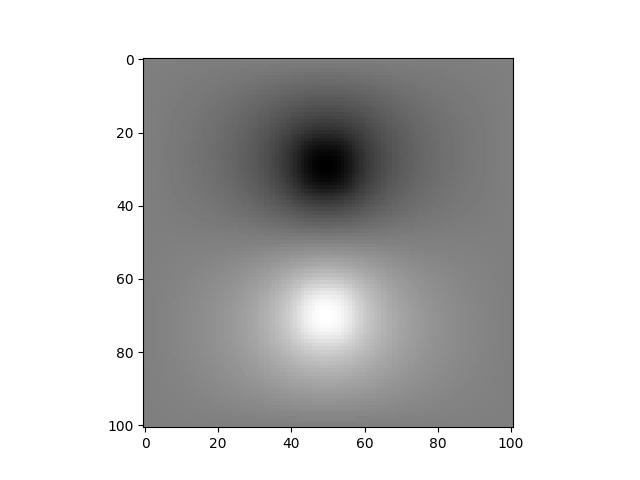
\includegraphics[scale = 1.0]{../Figure2};
    \caption{Solução para a equação de Poisson para densidades de carga na forma de retângulos}
    \caption{fig:solucao}
  \end{figure}

  Como comentários finais, o tempo de processamento do programa \texttt{4-poisson.py} é de 10 minutos e 43.358 segundos. Em contraste, o programa requerido na questão 3, a ser apresentado, fora escrito em C e seu tempo de processamento foi de 9.620 segundos!

  Apesar de uma pequena otimização feita (na função \texttt{swap} e como é utilizada), a diferença de tempo de processamento é claramento muito grande, mostrando a não eficiência da linguagem Python para processamentos pesados.

  \begin{figure}[h]
    \center
    \begin{tk3}
      \begin{tikzpicture}[node distance = 15mm, auto]
        \node (start) [startstop] {Program \texttt{4-poisson.py}};
        \node (constants) [process, below of = start, yshift = 2mm] {Define some constants for the programa: \texttt{a}, \texttt{delta}, \texttt{target}, \texttt{L $\leftarrow$ (M+1)a}};
        \node (initialize) [process, below of = constants, yshift = -3mm] {Initialize the matrix $\phi \texttt{[} \texttt{]} \texttt{[} \texttt{]}$ and the array $\rho$\texttt{[][]} (via (\ref{eq:3}))};

        % Whiles and loops
        \node (targetLoop) [decision, below of = initialize, xshift = -57mm, yshift = 10mm] {$\texttt{delta} > \texttt{target}$ ?};
        \node (forLoop) [process, right of = targetLoop, yshift = 0mm, xshift = 42mm] { \texttt{x = 0; while (x < L)} \\ \texttt{y = 0; while (y < L) } };

        \node (PhiPrime) [process, below of = forLoop, xshift = 10mm] {Calculate $\phi^\prime[\texttt{x}][\texttt{y}]$ via (\ref{eq:2})};
        \node (attXY) [process, below of = PhiPrime, yshift = 3mm] {\texttt{x = x + a} \\ \texttt{y = y + a}};
        \node (calcDelta) [process, below of = attXY, xshift = -10mm] {Calculate \texttt{delta} (\texttt{delta} = $max\abs{\phi^\prime - \phi}$)};
        \node (swap) [process, below of = calcDelta, yshift = 2mm] {Swap the elements of $\phi \texttt{[][]}$ and $\phi^\prime \texttt{[][]}$};

        \node (plot) [io, below of = swap] {Plot $\phi\texttt{[][]}$ as \textit{density plot}};
        \node (stop) [startstop, below of = plot, yshift = 4mm] {Finished};

        \draw [arrow] (start) -- (constants);
        \draw [arrow] (constants) -- (initialize);
        \draw [arrow] (initialize) -- (forLoop);
        \path [line]  (targetLoop) -- node[anchor = south] {no}(forLoop);
        \path [line]  (targetLoop) -- (-7.54, -5.1) -- node[anchor = east]{yes}(-7.54, -12.1) -- (plot);

        \draw [arrow] (forLoop) -- (PhiPrime);
        \draw [arrow] (PhiPrime) -- (attXY);
        \path [line] (attXY)  -- (-2.6,-7.85) -- node[anchor = east]{inside loop}(-2.6, -5.6);

        \path [line]  (forLoop) -- (5, -5.1) -- node[anchor = west]{loop finished}(5, -9.25) -- (calcDelta);
        \draw [arrow] (calcDelta) -- (swap);
        \path [line]  (swap) -- node[anchor = south]{verify condition}(-5.64, -10.6) -- (targetLoop);

        \draw [arrow] (plot) -- (stop);
      \end{tikzpicture}
    \end{tk3}
    \caption{Flowchart of the program \texttt{4-poisson.py}}
  \end{figure}



\end{document}
